\chapter{Introduction}
\label{ch:intro}

% Robin's comments
    % more structure: subsections, giant block of text.
    % better argument for your case
    % the result of the arguments should be the research questions
    % some alternatives of the research questions

% \todo[inline]{should I talk about information need of users and the fundamentals why recommender systems are a service and what they are? I don't do that here at all.}
% \todo{research context}

After a fast development in creating ``smarter'' digital systems, more and more decisions are being delegated to algorithms. Having observed the evolution, influence, and consequences of these AI-supported systems over time, concerns have been grown in the public discourse about ethical issues and the potential harms of these systems to individuals and society. 
% Machine learning is and continues to be one of the main pillars of these systems.
 
Recommender systems are one of the most pervasive applications of AI/machine learning. They play a pivotal role in connecting users to relevant items or content throughout the web. Not only do users rely heavily on these systems, but also other parties such as content producers, sellers, or information providers. Although these systems are intended to assist people in different tasks, they can risk implicit or explicit discrimination against individuals or groups, especially marginalized groups. Consider a recommender system suggesting job opportunities to job seekers. Discriminatory recommendations in these systems could mean that men and women with similar qualifications don't get recommendations for jobs with equal rank and salary.
%they can potentially cause implicit or explicit

% \todo[inline]{is a job recommendation scenario out of context?}
% Many online... is redundant.

%Many online platforms attempt to connect job opportunities and job applicants in some way.Sometimes they are professional networks with a job-seeking component such as Xing and LinkedIn, or they might have been designed only for employment seeking.

For example, suppose more women apply for lower-paying jobs on a given job-seeking website, and the recommendation algorithm learns the correlation between demographic information and job salaries. Jobs with lower salaries or ranks might show up more often in the recommendations to women and jobs with better salaries and higher ranks will be recommended to men. Basileal et al. (2021) \cite{Korolova2021JobAds} demonstrate this issue in the Facebook's ad delivery system and how demographic information causes the system to discriminate against women regardless of their qualifications.

%not recommender system's fault!
% In another real-world example, Brian Stauffer (2018) from Human Rights Watch reports similar discrimination against women in the job market \cite{HRW2018ads}. They analyzed over 36,000 job advertisements posted between 2013 and 2018 on Chinese recruitment and company websites and social media platforms. Many of the ads specify a requirement or preference to hire men regardless of other qualified women candidates. Some job posts require women to have certain physical attributes – with respect to height, weight, voice, or facial appearance – that are irrelevant to job duties.

% ali2019JobDiscrimination
% when they get similar recommendations, it is just because of their demographic information not because of their qualifications.

Now, consider a loan recommender system that suggests loans to lenders to support. Many online platforms attempt to connect small businesses or entrepreneurs in need of loans to lenders or donors, such as Kiva.org or DonorsChoose.org. Discriminatory recommendations in these systems could mean that, for instance, more attractive, lighter-skinned, and less obese borrowers are favored (discussed by Christina Jenq et al. (2015) \cite{JENQ2015234}), and their loans get funded faster.

There are several ways that different biases can creep into recommender systems. Reflection of societal and historical prejudices in datasets, lack of data on minority groups or any problem in data collection, and lack of suitable model designs and evaluation methods are among the underlying reasons for unfairness in these systems. A system needs to defend against these biases in recommendation output, even biases that arise due to behavioral differences. For example, male users might be more likely to apply optimistically for high-paying jobs compared to women. These differences reflect how these biases might have been internalized in people in the society and their behavior which may lead to discrimination in job recommendation. 


% \section{Running example}
% \todo{expand on it}

% \todo[inline]{
% Microlending is the provision of small and low-interest loans (as little as \$25) to low-income individuals or small-scale entrepreneurs from under-developed countries \cite{yunus1998banker}. The extremely poor people in rural areas often lack collateral, steady employment, or a verifiable credit history, hence they cannot get access to financial services. Under such circumstances, microlending has attracted an increased attention in the last decade \cite{chen2017microfinance}, providing impoverished entrepreneurs an opportunity to start their own businesses as well as avoid the vicious cycle of debt.

% One of the leading international microlending organizations, Kiva Microfunds (Kiva.org), has crowd-funded about 3 million borrowers with \$1.27 billion USD as of February 2019 \cite{kiva}. Kiva does not collect interest but provides an intermediary service for lenders and borrowers, as illustrated in Figure \ref{fig:kiva_process}. Borrowers from over 80 countries, divided into 8 regions by Kiva, post their applications for loans on the website for lenders to support. Lenders browse and crowd-fund the loans in the increments of \$25 or more. }

% Consider a loan recommender system that suggests loans to lenders to support. There are many online platforms attempting to connect small businesses or entrepreneurs who have requested for a loan to lenders or donors in some way. Discriminatory recommendations in this system could mean that for instance, more attractive, lighter-skinned, and less obese borrowers are favored \cite{JENQ2015234}, and their loans get funded faster. 
% Or when they get similar recommendations, it is just because of their similar demographic information not because of reasons they have provided about why they need the loan.

% The system would therefore need to defend against biases in recommendation output, even biases that arise due to behavioral differences: for example, certain regions in the world are more favored due to the historical or political relationships of the countries where the lenders and borrowers reside. Therefore, certain borrowers unjustly get a high exposure to the lenders and the others might not get any visibility at all. And due to the formed positive feedback loops, this gap might get wider over time, resulting in ignoring certain user subgroups.

% Consider a recommender system suggesting job opportunities to job seekers. Many online platforms attempt to connect job employments and job applicants in some way. Sometimes they are professional networks which have a job-seeking component such as Xing and LinkedIn, or they might have been designed only for employment seeking.

% Discriminatory recommendations in this system could mean that men and women with similar qualifications don't get recommendations of jobs with similar rank and salary. Or when they get similar recommendations, it is just because of their demographic information not because of their qualifications. For examples, if there are more women on a job recommendation website and they all apply for secretarial jobs, these jobs might show up in the recommendations of women who are looking for CEO jobs. On the other side of the coin, jobs with better salaries and higher ranks will be recommended to men regardless of their qualifications. The system would therefore need to defend against biases in recommendation output, even biases that arise due to behavioral differences: for example, male users might be more likely to click optimistically on high-paying jobs. \todo{more clarifications?}

% \section{Sources of unfairness in recommender systems}

% % potential underlying reasons for recsys to be unfair
% Multiple underlying reasons cause the recommendation algorithms to be unfair. For example, if recommender systems are trained on biased data, the outcomes might get biased, a.k.a. "garbage in, garbage out."

% These algorithms might also propagate the existing biases in the data \cite{barocas2016big}. For example, recommender systems increase the popularity of items by just presenting those items to the users. 
% It is known that these systems affect the users’ opinion, and hence, their ratings of items \cite{Cosley2003Influence}. Thus, a user’s rating of an item is either their intrinsic preference or the influence of the recommender system on the user. Users are more likely to click on the items that recommender systems deliver to them. This phenomenon is called presentation bias \cite{baeza2018bias}. 

% Over time, items gain even more popularity as they are shown to users, up to the point that less popular items are not recommended at all. Due to the positive feedback loop, the item space shrinks, and the recommendation lists become too homogeneous \cite{Chaney2018Homogeneity}. The formed \textit{filter bubble} might be harmful or unfair to users as users' choices become limited and homogeneous, preventing them from novel content or ideas.

% A real-world example of the harms that filter bubbles cause; is the influence of the news feeds on people's minds that can eventually lead to political polarization~\cite{HONG2016777}. Not only is this issue discriminatory towards users, but it is also unfair to (content) providers as a small group of them gain unfairly high visibility while the others are systematically pushed away. In a music streaming platform, this issue could affect the livelihood of musicians. In Algorithms of Oppression, Sofiya Noble \cite{noble2018algorithms} discusses this issue in personalized search through real-world examples and people's experiences. The author later, discusses how popularity bias in Yelp along with other factors such as private interests in promoting certain sites, along with the monopoly status of a relatively small number of Internet search engines, can potentially lead to racial discrimination, especially businesses owned by women of color.

% Over-personalization in Youtube's recommendation algorithms has also caused harm to suicidal teenagers by showing them similar videos on different ways of committing suicide.
% This type of bias occurs because users are more likely to interact with items that the system presents to them. 
    
% The first issue here is the item selection by the recommender system here and whether it will contribute to unfairness to any of the stakeholders. We have addressed how to mitigate this issue in Chapter \ref{fairness} in the pre-processing section \todo[inline]{preprocessing section}. 
    
% The second issue is that presentation bias, can lead to a form of positive feedback loop, in which presented items gain more popularity since they are more likely to be interacted with. This leads to greater bias towards presenting the items when the popular items are promoted more at the cost of other items. Presentation bias and the created feedback loop not only magnifies the initial differences between items' popularity but also it makes it hard for new providers to attract the attention of users to their products/items in a system with this type of bias.
    
% For example, in the microlending case, if the system doesn't recommend loans from a specific geographical region because on average the requested loans from this region are risky (their borrowers are less likely to return the loan), not only the current good borrowers (the borrowers who are more likely to return the loan) from that region are affected, but also the future good borrowers. This positive feedback loop reinforces over time until that region is completely ignored by the system.

\section{Fairness-Aware Recommender Systems}

Disregarding the societal impacts and ethical consequences of recommendation algorithms in different applications leads to algorithm designs that are unfair or harmful to their users. In recent years, the topic of fairness in machine learning has gained the attention of a multi-disciplinary community from computer scientists, social scientists to legal scholars. Thus as a response, recent research has shifted from design of algorithms optimizing for accurate outcomes to ones that also consider algorithms' social impacts. 
% such as representational or distributional harms. %accurate outcomes 

The problem of mitigating unfairness in recommender systems has unique challenges that set it apart from general machine learning fairness problems: (a) the multi-stakeholder nature of these systems and (b) the centrality of personalization and its trade-off with fairness goals. These two unique properties prevent the researchers from directly translating the proposed solutions and common techniques in machine learning fairness to recommender systems. In the following sections, we dive into each of these two points separately.


\subsection{Fairness in Multi-stakeholder Systems}

Recommender systems are often multi-stakeholder settings with users or consumers (of recommendations), providers or producers (of content/items), or other parties involved in systems transactions. Fairness concerns might arise for any of these stakeholders, such as consumers, referred to as \textit{consumer-side fairness} concerns, or providers, referred to as \textit{provider-side fairness} concerns, or other stakeholders.

As an example, a system might be discriminatory towards certain job-seekers (consumers), such as women, by presenting them the recommendations of lower-paying job opportunities based on their demographic information, or it could be unfair to certain businesses (providers), such as start-ups, by not giving them enough visibility to the best candidates. In certain applications, these concerns might need to be addressed at the same time, but achieving universal fairness for all is impossible \cite{friedler-impossibility-2021}. So, we might need to prioritize fairness concerns across different stakeholders.


\subsection{Personalization versus Fairness}
% what accuracy is? and what word should we replace it with?
% In machine learning algorithms, achieving optimum accuracy by itself is impossible and might not even be desirable!

% I think you need to start with definitions: first, fairness. What do you mean? I would say the definition is something like: “The output of the system conforms to some normative distributional properties with respect to particular stakeholders.” Next, accuracy. “A system gives accurate recommendations if it can, on average, reproduce the preferences of users expressed in historical ratings data.” Don’t rely on people’s common-sense ideas of these terms, since you really mean something quite specific.

% With definitions in place it is easier to describe the tension between them: the historical preferences of users might not match the desired normative properties; the historical ratings of users are themselves only uncertainly related to users’ preferences; the historical ratings data is contaminated with various kinds of biases; the desired distributional properties work to the benefit of subgroup but the accuracy measure is averaged over all users; etc.

Traditionally, the main goal of a recommender system is personalization. In other words, recommender systems strive to present items to the users that are tailored to each user's taste and are more likely to be interacted with. To achieve personalization, these systems utilize users' historical log data to produce accurate recommendations. A system has high \textit{accuracy}, if it can, on average, reproduce the preferences of users expressed in historical ratings data.

A system is \textit{fair} if the output of the system conforms to some normative distributional properties with respect to particular stakeholders. Achieving a balance between fairness and accuracy as defined previously is challenging due to their intrinsic tension. The major underlying causes of this tension are as follows: the historical preferences of users might not match the desired normative properties; the historical ratings of users are themselves only uncertainly related to users’ preferences; the historical ratings data is contaminated with various kinds of biases; the desired distributional properties work to the benefit of subgroup but the accuracy measure is averaged over all users; etc. Below, I discuss an example for each cause.
% \todo[inline]{the topics needs to change - no time though :|}


% Based on this definition, achieving optimum accuracy by itself is impossible because the historical preferences of users might not match the desired normative properties. 

% Additionally, optimizing for accuracy might reinforce the popularity bias or some consumer-side unfairness. The following sections discuss how optimizing for accuracy can lead to user dissatisfaction and why we might need to balance accuracy with other system goals, such as fairness.

% \vspace{0.25cm}
% \noindent \textbf{(\romannum{1}) Fairness}
% \vspace{0.25cm}


% \subsection{Impossibility of Ideal Accuracy}
\vspace{0.25cm}
\noindent \textbf{(\romannum{1}) Impossibility of Ideal Accuracy}
\vspace{0.25cm}

Recommender systems recognize the more general patterns in the data and use this information to predict users' rating behavior for recommendation generation. These general patterns are based on historical logged user interactions with the system. Therefore accuracy for recommender systems is fidelity to historical patterns in the data and the ability to reproduce users' exact preferences. 

However, human behavior is always associated with some degree of uncertainty (as Hill et al. (1995) explains in \cite{hill1995recommending}), which will lead to deviation from perfect accuracy. This uncertainty might originate from the natural variability of human decision-making, or it might be system-induced. Users' rating behavior is inconsistent, and their preferences are not fixed. Said et al. (2012) \cite{Said2012MagicBarrier} introduces and discusses the concept of the \textit{magic barrier} in recommender systems, a barrier caused by variability in user behavior which prevents the model from reaching an ideal accuracy. Besides the behavioral inconsistency, users' tastes might evolve as they consume the recommendations. McAuley et al. (2013) \cite{McAuley2013expertise} discuss how user's ratings of beers change as their palate tastes more complicated tastes over time. 

% \todo[inline]{what the users want and what they click on is different?}
%historical logged user


% In this case, recommender systems generate recommendations according to the general patterns of users interests. 

To improve accuracy, recommender systems might need to model these temporal and dynamic changes. Additionally, recommender system models built on general patterns in the data capture mainly the long-term interests of users and might disregard users' short-term needs and interests. Many researchers, including Adomavicius et al. (2011) \cite{Adomavicius2011context}, have attempted to use contextual information to account for these changes.

In some cases, due to technical limitations or lack of data, the system fails to present users their items of interest, so users might end up clicking on the items that are not reflective of their interest. This data might enter the training data and bias the input for the subsequent iterations. The points mentioned above are just a few examples of underlying confounding factors behind variability in user behavior that make the prediction task challenging in these systems.

Even if the users' behavior is consistent and ideal accuracy is reachable, users' preferences might not conform to fairness concerns. This might be because users are inherently biased or simply because users are unaware of the unfairness in a system. As an example, Kiva.org's lenders might not be aware of the unprivileged borrowers in the system. Therefore, supporting loans only based on their preferences might further exacerbate the unfairness of capital distribution in the system.

% This is partly because users' 
% to keep up with the variability in users' rating behavior
% Users' preferences are inconsistent.
%These changes are hard to predict as there are many underlying confounding factors involved in them.

%  Some authors speculated that we may be reaching
% some Magic Barrier where this variability prevents us from getting much more accurate

% In practice, it is hard to predict the information need of users at each point in time. 
% In fact, users themselves might not even know what they want. For example, It would be odd to think that every time a user opens a music streaming platform, she will exactly know the songs she wants to play. So, achieving ideal accuracy is unlikely in spite of optimizing the objective function to increase it.

% For example, when you want to listen to music, a lot of the times you don't think about the songs you exactly want to listen to. You might not want to listen to what you were listening before. Therefore, we can never achieve perfect accuracy and presenting accurate recommendations to the users is a myth.

% Below are some examples of the potential biases that increasing accuracy causes for consumers and providers.
% \todo[inline]{check all the biases mentioned before..}

\vspace{0.25cm}
\noindent \textbf{(\romannum{2}) Accuracy and Data Imbalance}
\vspace{0.25cm}
% \subsection{Accuracy \& Data Imbalance}

The collected data used for training recommendation models might not reflect the diversity in the society due to various reasons such as biases in data collection or simply lack of online participation from minority groups. These issues can create data imbalance leading to accuracy imbalance between the majority user group(s) for whom we have more data versus minority groups with less data. Since accuracy-based metrics are aggregated over all the users, they may fail to capture the accuracy for different user subgroups in a system. Usually, accuracy reflects the quality of the recommendations that the majority of the users experience regardless of other minority groups' experience. The error disparity for different user groups is considered a type of unfairness and trying to balance it is of interest for the research community \cite{ekstrand2018all,yao2017beyond}.

% Therefore, minority groups might not receive a high-quality service in the system.

% These metrics are usually averaged over all the user base and skewed towards the majority user group.   So, having a discrepancy in recommendation quality for different user groups is a type of unfairness in recommender systems and reaching to balance it, is of interest for the research community \cite{ekstrand2018all,yao2017beyond}.

\vspace{0.25cm}
\noindent \textbf{(\romannum{3}) Accuracy and Popularity Bias}
\vspace{0.25cm}
% \subsection{Accuracy \& Popularity Bias}
% how is accuracy and popularity related
% \todo[inline]{define accuracy}

Recommendation datasets are usually intertwined with popularity bias \cite{celma2008hits,lee2014fairness}. Striving to reach high accuracy will often lead to reinforcing popularity bias~\cite{barocas2016big}. It is known that these systems affect users’ opinions, \cite{Cosley2003Influence}. Thus, a user’s rating of an item might be their intrinsic preference, or based on the influence of the recommender system, or a combination of both. Users are more likely to click on the items that recommender systems deliver to them. This phenomenon is called \textit{presentation bias} \cite{baeza2018bias}.

Over time, items gain even more popularity as they are shown to users, up to the point that less popular items are not recommended at all. Due to this positive feedback loop, the item space shrinks, and the recommendation lists become too homogeneous \cite{Chaney2018Homogeneity}. The formed \textit{filter bubble} might be harmful or unfair to users as users' choices become limited and homogeneous, preventing them from receiving novel content or ideas. A real-world example of the harms that filter bubbles cause for users is the influence of the news feeds on people's mindset that can eventually lead to political polarization~\cite{HONG2016777}.

% These algorithms might also propagate the existing biases in the data \cite{barocas2016big}. For example, recommender systems increase the popularity of items by just presenting those items to the users.

% Not only is this issue discriminatory towards users, but it is also unfair to (content) providers as a small group of them gain unfairly high visibility while the others are systematically pushed away. 
Not only the consumers of recommendations will be affected, but the item providers might also suffer from discrimination. Popularity bias leaves less popular (item) providers with fewer consumer exposure opportunities, pushing them away from the system. This unjust exposure can affect their livelihoods. In a music streaming platform, this issue could affect the musicians income. 

The unfairness caused by systems is not equally harmful to that system's users. It usually puts a greater burden on the protected groups, particularly those who sit at the intersection of multiple protected attributes, such as ``new'' businesses owned by ``women'' of ``color''. In \textit{Algorithms of Oppression}, Sofiya Umoja Noble (2018) \cite{noble2018algorithms} discusses this issue in personalized search through real-world examples and people's experiences, including how popularity bias in Yelp along with other factors such as private interests in promoting certain sites, as well as monopoly status of a relatively small number of Internet search engines, can potentially lead to racial discrimination, especially businesses owned by women of color.

Popularity bias in the input data can lead to defective power dynamics in the user subgroups and influence the overall recommendations. As an example, Eskandanian et al. \cite{Eskandanian2019power} discusses how this issue can cause the preference of 95\% the users to be overshadowed by only the preference of 5\% of influential users who have rated mostly popular items (consumer unfairness).

Using accuracy as the only measure to optimize might even be undesirable or unsatisfactory to one or all the stakeholders of a recommender system. This is because increasing accuracy, without considering other goals and the potential causes of harm, can contribute to introducing and propagating biases or even reinforcing some of the existing biases in the system, such as popularity bias, positive feedback loops, filter bubbles, miscalibration error, over/under estimation of the predictions, etc. 


% Recommendation datasets are usually inter-weaved with popularity bias. Striving to reach a high accuracy will lead to reinforcing popularity bias as well. Over time, this bias gets even worse due to the effect of positive feedback loops in the system.

% As a result, popular items will gain more popularity and will be recommended more often. 
% Therefore users will receive more and more homogeneous recommendations over time. The created filter bubble and presenting users with limited options is unsatisfactory to users. The previous research in the literature shows that increasing diversity in the recommendations increases user satisfaction, while we know diversity has a trade-off with accuracy. Aside from that, filter bubbles implicitly force users to consume the same content which can have harmful social impacts (polarizing the society based on political views, or recommending more violent videos to kids after watching only one video with the same content). 

% \subsection{Balancing Accuracy and Fairness}
\vspace{0.25cm}
\noindent \textbf{(\romannum{4}) Controlling the Trade-off between Accuracy and Fairness }
\vspace{0.25cm}

Despite all the previously mentioned issues about the accuracy/fairness trade-off and the need to consider non-accuracy goals, accuracy still has the highest priority. This priority is because high accuracy is deemed equal to high personalization, which is the core of recommender systems. Additionally, accuracy is considered to be strongly tied with user satisfaction in the system, which brings more revenue to e-commerce recommender systems. %compared to other beyond accuracy metrics.

% and also because compared to other goals like fairness or diversity, accuracy is financially more beneficial and hence necessary for the survival of the commercial recommendation systems (e-commerce websites).

Although, since the end goal for recommender systems is to serve its users and increase their satisfaction, any potential harm in the system should be prevented as much as possible, and the discrimination against its users should be mitigated. However, achieving universal fairness is impossible. In some application areas, certain aspects of fairness concerns are more important than others. In other applications, unfairness towards some stakeholders might have a higher stake compared to other stakeholders. For example, in the Kiva application, unfairness towards the lenders is less likely than toward borrowers. Therefore, fairness objectives for stakeholders should be meticulously picked and prioritized according to the fairness goals, the application, and the context.

Integrating and operationalizing a goal such as fairness to the system is essential but challenging, mainly because fairness can have significant trade-offs with accuracy and because achieving fairness for all stakeholders at the same time is impossible. Throughout this dissertation, I study the trade-off between accuracy and fairness in two different contexts where fairness has high stakes. I propose empirical solutions to control this trade-off and to find a sweet spot between the two competing goals. 

% \todo[inline]{add this => However, optimizing recommendation accuracy often comes at the expense of provider fairness, due to various biases present in recommender systems, including popularity bias \cite{celma2008hits,lee2014fairness}, and user-base composition \cite{lin2019crank, yao2017beyond}. Research in provider fairness is therefore generally concerned with improving the tradeoff between fairness and accuracy, or in other words, increasing the amount of fairness that can be gained for a given degree of accuracy loss.
% }

% \begin{comment}
% % bit and pieces
% Although increasing accuracy for better personalization can be a double edged sword. 
% On the one hand, accuracy is known to be strongly tied with user satisfaction and is financially conducive for the system. On the other hand, increase in accuracy might contribute to

% The end goal for the system is to serve users and benefits them. While in many cases, due to biases in the data (such as popularity bias) or the bias propagation over time, etc. more than a certain level of accuracy will become harmful to users from other aspects. Some of these other aspects are measures by beyond-accuracy measures such as diversity, fairness, serendipity.
% The previous research in the literature shows that increasing diversity in the recommendations increases user satisfaction, while we know diversity has a trade-off with accuracy.

% These issue complicate the research problems more since, we need to understand these aspects of the problem in order to meticulously identify the context of the problem, the type of unfairness we can address, and the the family of solutions that we want to adopt in order to operationalize fairness in recommender systems.
% \end{comment}

% kiva? non-profit context? 

% how is this problem and set of solutions different than the ones that are proposed to solve popularity bias?

\section{Contexts}
    
    We assess the unfairness of recommender systems and propose solutions to mitigate unfairness in these systems under two different contexts: Philanthropic and Streaming Media/E-commerce.

    \subsection{Philanthropic - Loan Recommendation}

        Online sites have become a significant avenue for people not only for shopping but for philanthropic activities. Kiva Microloans is a non-profit organization that operates a crowd-sourced micro-lending platform. Microlending is the provision of small and low-interest loans (as little as \$25) to low-income individuals or small-scale entrepreneurs from under-developed countries \cite{yunus1998banker}. Extremely poor people in rural areas often lack collateral, steady employment, or a verifiable credit history, hence they cannot get access to financial services. Under such circumstances, microlending has attracted increased attention in the last decade \cite{chen2017microfinance}, providing impoverished entrepreneurs an opportunity to start their own businesses as well as avoid the vicious cycle of debt.
        
        %  Kiva Microfunds (Kiva.org) is one of the leading international micro-lending organizations that has crowd-funded about 3 million borrowers with USD \$1.27 billion as of February 2019 \cite{kiva}. Kiva does not collect interest but provides an intermediary service for lenders and borrowers, as illustrated in Figure \ref{fig:kiva_process}. Borrowers from over 80 countries, divided into 8 regions by Kiva, post their applications for loans on the website for lenders to support. Lenders browse and crowd-fund the loans in the increments of \$25 or more.
        
        % Kiva as a micro-lending organization, uses crowd sourcing to provide access to capital for individuals and entrepreneurial groups, especially in the developing world, who are otherwise under-capitalized.
        % with the goal of financial global inclusion. 
        
        Kiva partners with local organizations in countries across the globe and, since its founding, has lent \$1.46 billion to 3.4 million borrowers in 77 countries with the support of 1.9 million lenders. Information about lending opportunities is listed on Kiva's site for a fixed period and promoted to its lenders through various means. A typical lender will contribute only a fraction of the total amount (as low as \$25) for any one loan, but may support multiple loans at any one time. As with any lending transaction, there is risk that the borrower will not repay, but this is rare in Kiva where the repayment rate is approximately 96\%. Lenders do not get any interest on their investments so supporting a Kiva borrower is essentially a philanthropic act.
        
        Therefore, the main sides of the interaction are the borrowers, generally developing-world entrepreneurs who seek small amounts of capital to enhance their business capacity, and lenders, who are the application's end-users, as illustrated in Figure \ref{fig:kiva_process}. Note that the borrowers are the providers or the producers of the items/loans, and the lenders are the receivers or users of the recommendations. Kiva's mission emphasizes equitable access to capital for its borrowers, who generally cannot make use of traditional forms of banking and lending~\cite{Choo_understanding_kiva}. In this situation, a loan recommender system is intended to lower the search costs of its users (lenders) by finding borrowers whose goals and needs appeal to them. Several provider-side fairness concerns arise in this recommendation context, but no consumer-side fairness has risen as a concern so far.
        % \todo[inline]{provider-side and consumer-side fairness aren't defined}
        
        \begin{figure}[htb]
        %\vspace{-0.25cm}
        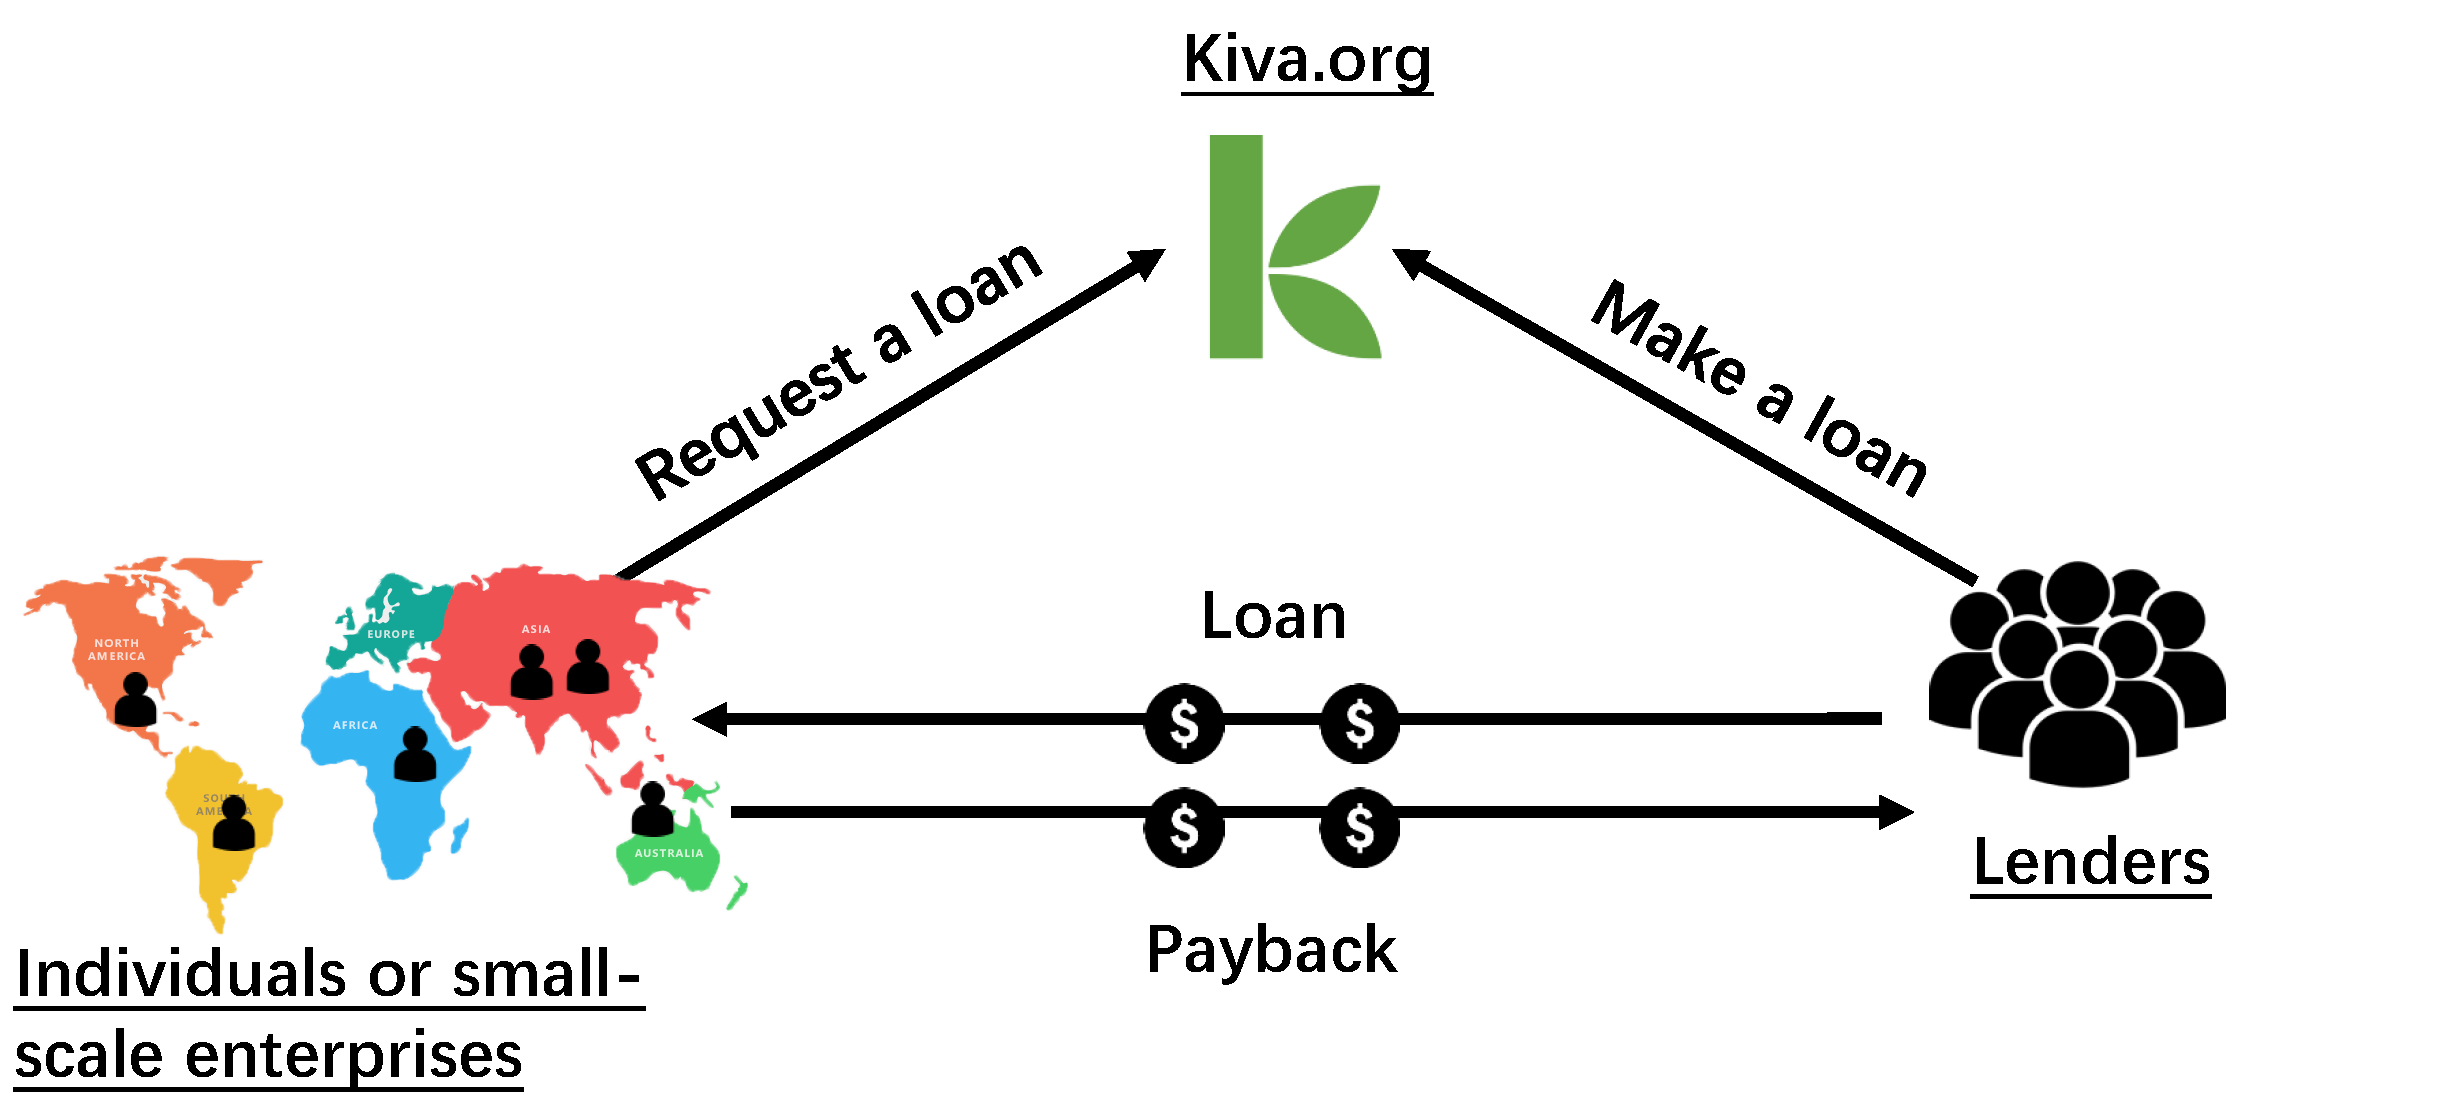
\includegraphics[width=0.98\columnwidth]{imgs/far/microlending.png}
        %\vspace{-0.25cm}
        \caption{Kiva.org provides an intermediary service for lenders and borrowers.}
        \label{fig:kiva_process}
        \end{figure}
        
        
        One key provider-side concern arising from Kiva's mission of supporting worldwide access to capital is that the geographic imbalances in users' preferences may manifest themselves in the disproportionate representation of certain countries or regions in recommendation lists. This could give rise to a positive feedback loop, as the recommended items are more likely to be supported, and thus the lending becomes even more highly concentrated. A similar kind of imbalance may arise with respect to different industries or economic sectors. Thus, we can identify at least two fairness concerns within this recommender system: equity in geographic distribution of capital \cite{liu2019personalized}, and equity across economic sectors \cite{sonboli2020opportunistic} which will be explained in detail in Chapter \ref{ch:fairness_postproc}. Other provider-side fairness concerns might arise in this context, e.g., the loan amount (loans with higher amounts get funded more slowly), but these are outside the scope of this thesis.
        
        % \todo[inline]{move this earlier}
        We situate our research within the organizational context of Kiva Microloans. This is a compelling case study to explore recommendation fairness since its fairness requirements are driven by internal needs surrounding its philanthropic mission, rather than external demands such as regulatory requirements found in financial services or employment, etc. A regulatory environment is more likely to provoke a defensive response related to fairness questions, which tends to hamper robust discussion of fairness properties in existing systems~\cite{chen2018fair,holstein2019improving}. A real-world example of Kiva's fairness-aware recommendations is depicted in Figure \ref{fig:kiva_underbanked}.
        
        
        \begin{figure}[htb]
        %\vspace{-0.25cm}
        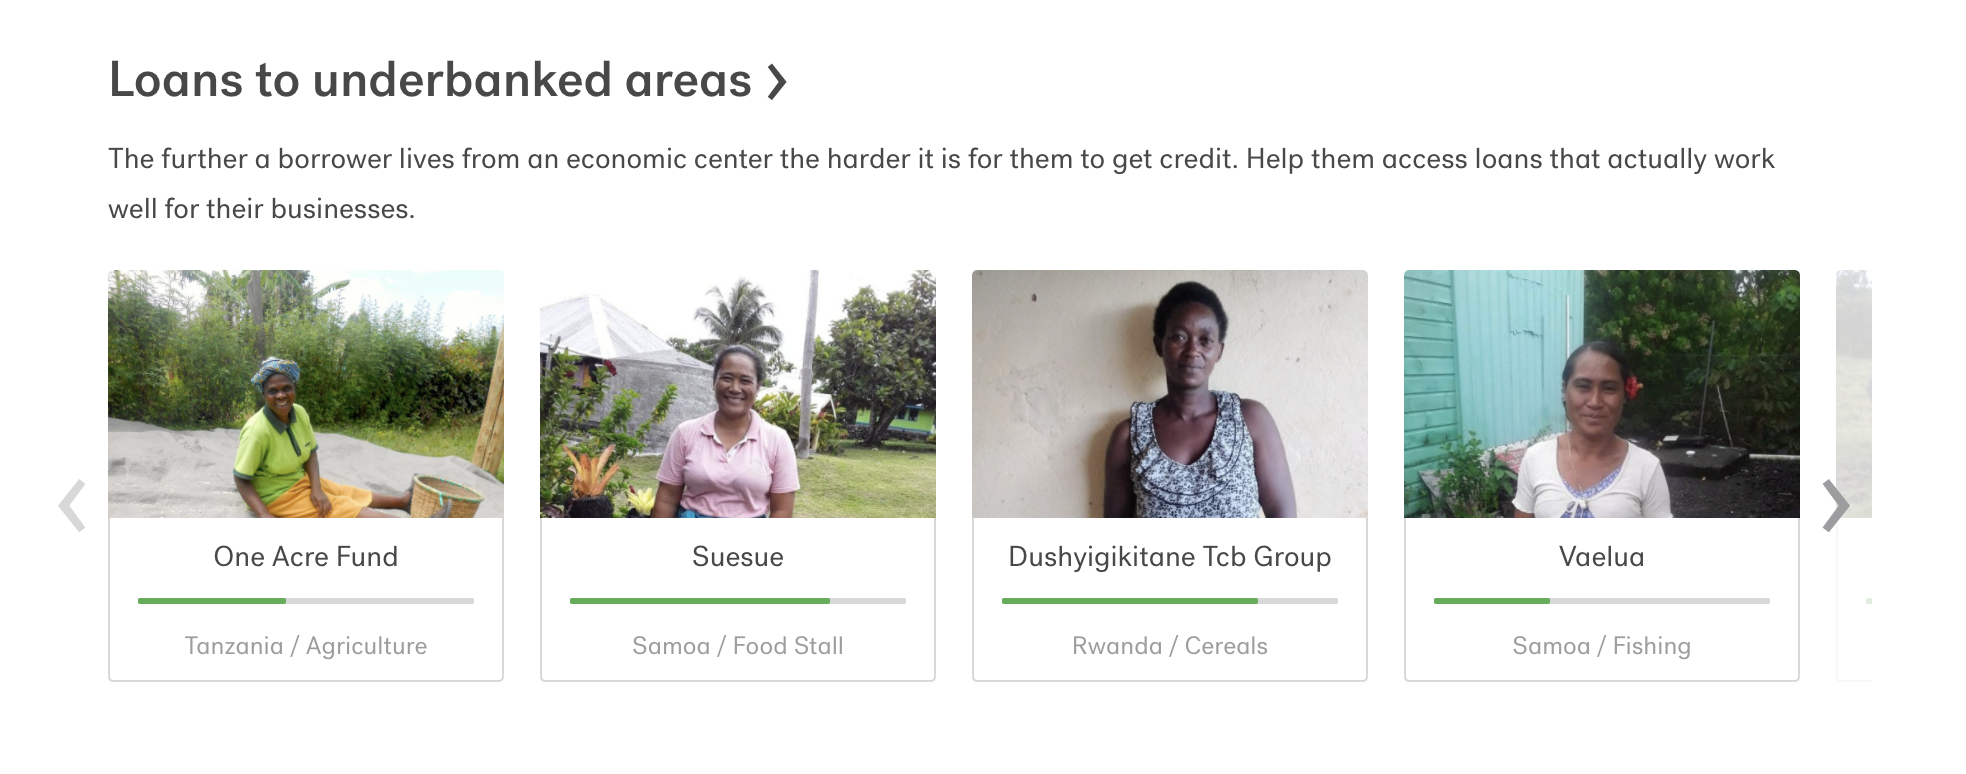
\includegraphics[width=0.98\columnwidth]{imgs/far/underbanked_areas.png}
        %\vspace{-0.25cm}
        \caption{Kiva.org provides fairness-aware recommendations.}
        \label{fig:kiva_underbanked}
        \end{figure}
        
        In addition, because of its philanthropic mission, it is reasonable to expect that Kiva's users will be receptive to fairness-oriented interventions. Finally, as a hybrid organization, embodying the characteristics of a nonprofit with the characteristics of a financial services institution, research embedded with Kiva is well-situated to have a broader and more generalizable impact across genres of institutions and sectors.
    
        % Loan recommendation, as in the case of Kiva is a suitable candidate for the exploration of recommendation fairness due to several reasons. One of them is that fairness requirements are driven by the internal needs surrounding Kiva's philanthropic mission to provide equitable access to capital for its borrowers regardless of their demographic information such as gender, the country of origin, etc., as well as other characteristics e.g. the economic sector for which they need the loan. Another reason reason on the suitability of Kiva is as follows: Kiva's users will be more receptive of the fairness-oriented interventions in recommendations due to its philanthropic nature whereas the users of a movie streaming website such as Netflix, might not care to be fair to the movie producers.
    

    \subsection{Streaming Media/E-commerce - Movie Recommendation}

        Streaming services for digital media consumption provide users with on-demand access to global content, connecting users with content creators, e.g., users and moviemakers on video streaming platforms like Netflix. Algorithmically generated recommendations power and shape the bulk of consumption patterns on such platforms. As Mehrotra et al. \cite{Mehrotra2018Towards} note, to maximize user satisfaction, streaming platforms that are optimizing for relevance could inadvertently be detrimental to exposure of the providers or content creators such as movie producers on the tail-end of the spectrum. As we have explained in the problem statement, optimizing only for relevance may lead to provider-unfairness, and consumer-unfairness.
        
        Therefore, streaming platforms carefully consider the influence of their recommendations on consumption patterns benefiting not only the users, but also creators, and the long-term goals of the platform itself. To better navigate such trade-offs between different stakeholder objectives, platforms are increasingly relying on multi-objective methods to jointly optimize multiple user-centric goals (e.g., engagement metrics like clicks, number of songs played, time spent), provider-centric goals (e.g., exposure) and platform-centric goals (e.g., fairness, discovery, diversity) \cite{mehrotra2020bandit}. In certain cases, aptly balancing such varied objectives makes it possible to obtain gains in both complementary and competing objectives.
        
        In this dissertation, we chose the movie recommendation context due to several reasons. Similar to the case of Kiva, fairness concerns regarding the exposure of the providers arise in these systems as well. We have addressed this issue in Chapter \ref{ch:fairness_postproc} in \cite{sonboli2020opportunistic,liu2019farpfar}.
        
        % \todo[inline]{cite dynamic fairness project}.
        
        Movie recommendation might not be an obvious candidate for the study of consumer-side fairness in recommender systems. Still, we used an approach similar to the method discussed by Yao, Sirui and Huang, Bert (2017) in \cite{yao2017beyond} to construct an artificial equity scenario within both MovieLens-1M and The Movies data for expository purposes only, with the understanding that real scenarios can be approached with a similar method. We chose MovieLens datasets due to the other following reasons: (a) MovieLens-1M is among the very few datasets with demographic information which makes it suitable for the use case of consumer-side fairness, (b) MovieLens-1M is a standard and commonly used dataset in the field of recommendation systems, and (c) generally, there is a lack of datasets in domains where fairness matters.


\section{Fairness Interventions in Recommendation Models}

    Fairness is a complex concept. It can have many different definitions under different contexts. More details on these concepts will be provided in Chapter \ref{ch:fairness}. In general, a system may have multiple \textit{fairness concerns}, particular aspects of its impact that may produce or perpetuate unfairness relative to a particular group measured in a specific way. This work concentrates on group fairness, focusing on increasing group fairness for under-privileged providers or consumers. %In other words, I intend to increase their exposure opportunities.
    
    % \todo[inline]{this term is not defined (fairness concerns)}
    After identifying the fairness concerns and defining them according to the context and application in use, it becomes possible to consider interventions in recommender systems to improve their fairness and performance. In doing so, it is worth keeping in mind the ``traps'' identified by Selbst et al. (2019) in \cite{selbst2019fairness}, possible hazards in applying fairness concepts in sociotechnical systems. Selbst and colleagues note that sometimes a technical fix is not always the most appropriate approach for problems of power imbalance and bias, and the failure to recognize this is defined as the \textit{solutionism trap}. There may be a wide variety of non-computational solutions to problems that surface themselves as unfair recommendations. Generally, three types of solutions have been proposed to operationalize fairness notions to mitigate unfairness: pre-processing, in-processing, and post-processing approaches.
    
    \textbf{Pre-processing} methods focus on compensating for the existing biases in a dataset, using different data collection enhancements to compensate for the biases that occur due to data imbalance. \textit{In-processing} approaches try to improve the fairness of results by integrating fairness notions into recommendation generation itself. \textit{Post-processing} approaches focus on modifying the outputs of algorithms to satisfy a fairness criterion. More details on these methods can be found in Chapter \ref{ch:fairness}. We propose one in-processing, and three post-processing approaches to improve the fairness-accuracy trade-off. Additionally, I will discuss the preliminary studies on a pre-processing method. More details are presented in Chapter \ref{ch:fairness_inproc}, and Chapter \ref{ch:fairness_postproc}. 
    % We run our experiments and analyze our results in the e-commerce and philanthropic contexts, which are explained in Chapter \ref{ch:methodology}.

%TODO check capital Chapter

% Throughout this dissertation, we propose different approaches to address achieving a better trade-off between accuracy and fairness. 

% For example, Kiva is a non-profit organization that operates a crowd-sourced microlending platform with the goal of financial global inclusion. In Kiva, the sides of the interaction are the borrowers, generally developing-world entrepreneurs who seek small amounts of capital to enhance their business capacity, and lenders, who are the application's end-users. A typical lender will contribute only a fraction of the total amount for any one loan, but may support multiple loans at any one time. Lenders do not get any interest on their investments and so supporting a Kiva borrower is essentially a philanthropic act. Kiva's mission emphasizes equitable access to capital for its borrowers, who generally cannot make use of traditional forms of banking and lending~\cite{choo2014gather}. Lenders are the users of the recommender system, which has the purpose of lowering their search costs in finding borrowers whose goals and needs appeal to them. 

% explaining the fairness issues
% Several provider-side fairness concerns might arise in this recommendation context.\footnote{Consumer-side fairness has not arisen so far as a concern in this application.} One key concern, arising from Kiva's mission of supporting world-wide access to capital, is that the geographic imbalances in users' preferences may manifest themselves in the disproportionate representation of certain countries or regions in recommendation lists. This could give rise to a positive feedback loop, as the recommended items are more likely to be supported, and thus the lending becomes even more highly concentrated. A similar kind of imbalance may arise with respect to different industries or economic sectors. Thus, we can identify at least two fairness concerns within this recommender system: equity in geographic distribution of capital \cite{liu2019personalized}, and equity across economic sectors \cite{sonboli2020opportunistic}.


\section{Research Questions}

%incomplete.. question and brief solution and the problems that it follows
The research questions that I seek to answer are as follows:
%TODO check I versus passive
\begin{itemize}
    \item (RQ1): How can we characterize the fairness/accuracy trade-off in different algorithms?
    % \todo[inline]{how does different algorithms compare (all rerankers), which algorithm should I use?}
    \item (RQ2): How can we incorporate fairness objectives into recommendation generation or post-processing to achieve better trade-offs? % far/pfar, ofair
    \item (RQ3): How can we extend these ideas to more complex scenarios involving multiple fairness concerns or requiring dynamic assessment of fairness opportunities? %dynamic fairness, multiple fairness concerns
    \item (RQ4): How can we ensure the reproducibility of the results and widen availability of fairness-aware techniques in recommender systems research? %librec
\end{itemize}


\section{Summary of Contributions}

My work here has primarily focused on developing recommendation approaches in which fairness metrics are jointly optimized along with recommendation accuracy. I have structured the problems and solutions to control and set the balance between accuracy and fairness. In other words, my goal is to improve group fairness while preserving accuracy as much as possible. Throughout the following work, I recognize all the stakeholders in a recommendation setting and propose solutions to improve fairness. I have used both error-based and exposure-based fairness metrics to assess unfairness of the results. 

I present the following contributions to the fairness-aware recommendation field. The first two contributions examine the first and second research questions. The third and fourth contributions investigate the third research question, and my contributions to the last project respond to the fourth research question.

\begin{itemize}
    \item \textbf{(Chapter \ref{ch:fairness_inproc}) Balanced Neighborhoods}:
    Here, I present an in-processing method to improve fairness while preserving as much accuracy as possible. Through introducing a regularization factor in the model, we provide a diverse neighborhood for each user. Diversity in every user's neighborhood ensures a less biased set of recommendations. Additionally, in his method, we can control the balance between fairness and accuracy via a hyper-parameter. Further, I define the concept of multi-sided fairness and demonstrate improvements in fairness for two sides of the recommendation setting: consumers and providers.
    % For more details please refer to Chapter \ref{ch:fairness_inproc}.
    
    \item \textbf{(Chapter \ref{ch:fairness_postproc}, Section \ref{sec:farpfar}) Fairness-Aware Recommendation Re-ranking (FAR) and Rersonalized Rairness-Aware Re-ranking (PFAR)}: 
    I describe two greedy re-ranking approaches here, both based on XQuAD (a method proposed by Santos et al. (2015)~\cite{santos2015search}, to increase diversity in lists for ranking methods). Both re-rankers are designed to increase group-based provider-side fairness and improve the fairness/accuracy trade-off. The developed methods here are purposed for a loan recommendation scenario, although they can be adapted to other contexts. 
    % This method is explained in details in Chapter \ref{ch:fairness_postproc}.
    
    \item \textbf{(Chapter \ref{ch:fairness_postproc}, Section \ref{sec:ofair}) Opportunistic Fairness-Aware Re-ranking (OFAiR)}:
    Here, I introduce the concept of opportunistic fairness. A novel method to improve personalization and fairness according to users' propensity to diversity in their recommendation lists. Additionally, I use a greedy re-ranking approach based on Maximal Marginal Relevance or MMR (a method presented by Xia et al. (2015)~\cite{xia2015learning} in the information retrieval field) to improve the accuracy/fairness trade-off for multiple aspects of fairness at the same time. 
    % This method is explained in details in Chapter \ref{ch:fairness_postproc}.

    % This post-processing approach is one of the few approaches that defines multi-aspect fairness and designs a method to improve different fairness goals of various providers in a simultaneous way. As an example, improving the visibility of impoverished loan borrowers with respect to different aspects such as: region of the world, their demographic information, loan amount, the economic sector, etc.
    
    % Users are not willing to experience diversity in every aspect of their recommendation. We detect the areas in which the users show willingness to see diversity and we consider them as opportunities to increase fairness without sacrificing much accuracy.
    
    \item \textbf{(Chapter \ref{ch:fairness_postproc}, Section \ref{sec:dynamicfair}) Social Choice for Re-ranking Under Fairness}:
    Here, I propose a novel framework for recommender systems called \textit{Social Choice for Re-ranking Under Fairness} (SCRUF). This framework is appropriate for dynamic environments where multiple fairness concerns matter. In this method, we use group-based exposure-based provider-side fairness definitions. 
    
    % This method is explained in details in Chapter \ref{ch:fairness_postproc}.
    %TODO make the title cases for all items consistent
    
    \item \textbf{(Chapter \ref{ch:librec-auto}) Standardizing and automating recommendation experiments via Librec-auto}: 
    Here, I present my contributions to \libauto{}, an open-source Python package incorporating different recommendation algorithms and evaluation methodologies. I have used \libauto{} throughout my dissertation to run experiments. 
    
    % For more details, please refer to Chapter \ref{ch:librec-auto}.
    
\end{itemize}



% 1) Can we maintain a high level of accuracy for the user base while increasing provider fairness? Or consumer fairness?

% 2) How can we control the accuracy trade-off better for providers? How to preserve accuracy while doing that? 

% 3) How can we control the accuracy fairness trade-off better for providers when addressing multiple fairness concerns? And can we use user propensities towards different categories to preserve accuracy as much as possible?

% 4) how can we achieve this balance dynamically?

% 5) What if we have data constraints? data minimization
% 6) Who controls the trade-off between accuracy and fairness? Should users have some agency over it? Should it be transparent to the users? Will re-rankers provide more transparency?


%%%%% incomplete


% This trade-off can have different underlying reasons. firstly, accuracy/personalization is a consumer-centric goal most of the time, and for example provider-side fairness is provider side. due to popularity bias, increasing personalization, might lead to less diversity for providers. and eventually less diversity for the consumers themselves. Achieving different goals at the same time might not be even possible. one other reason is the multi-party settings that recommendations offer, every one is striving to achieve what's best for them, and these goals might be competing. providers want one thing, the consumers want another thing. Therefore it's important to design methods to find a balance between these goals.


% \todo{mentioning that the cost of the data and EU rules, doesn't always allow up to gather more data, we do the data minimization then...}
% \todo{Do we need a summary of Contributions?}
% \todo[inline]{Do we need future work section?}

